\subsubsection{State}
\label{sec:world-state}

The \textbf{World State}, referred as the \emph{state}, in its simplest
definition, is a mapping between account addresses and account states.

\begin{figure}[h]
  \centering
  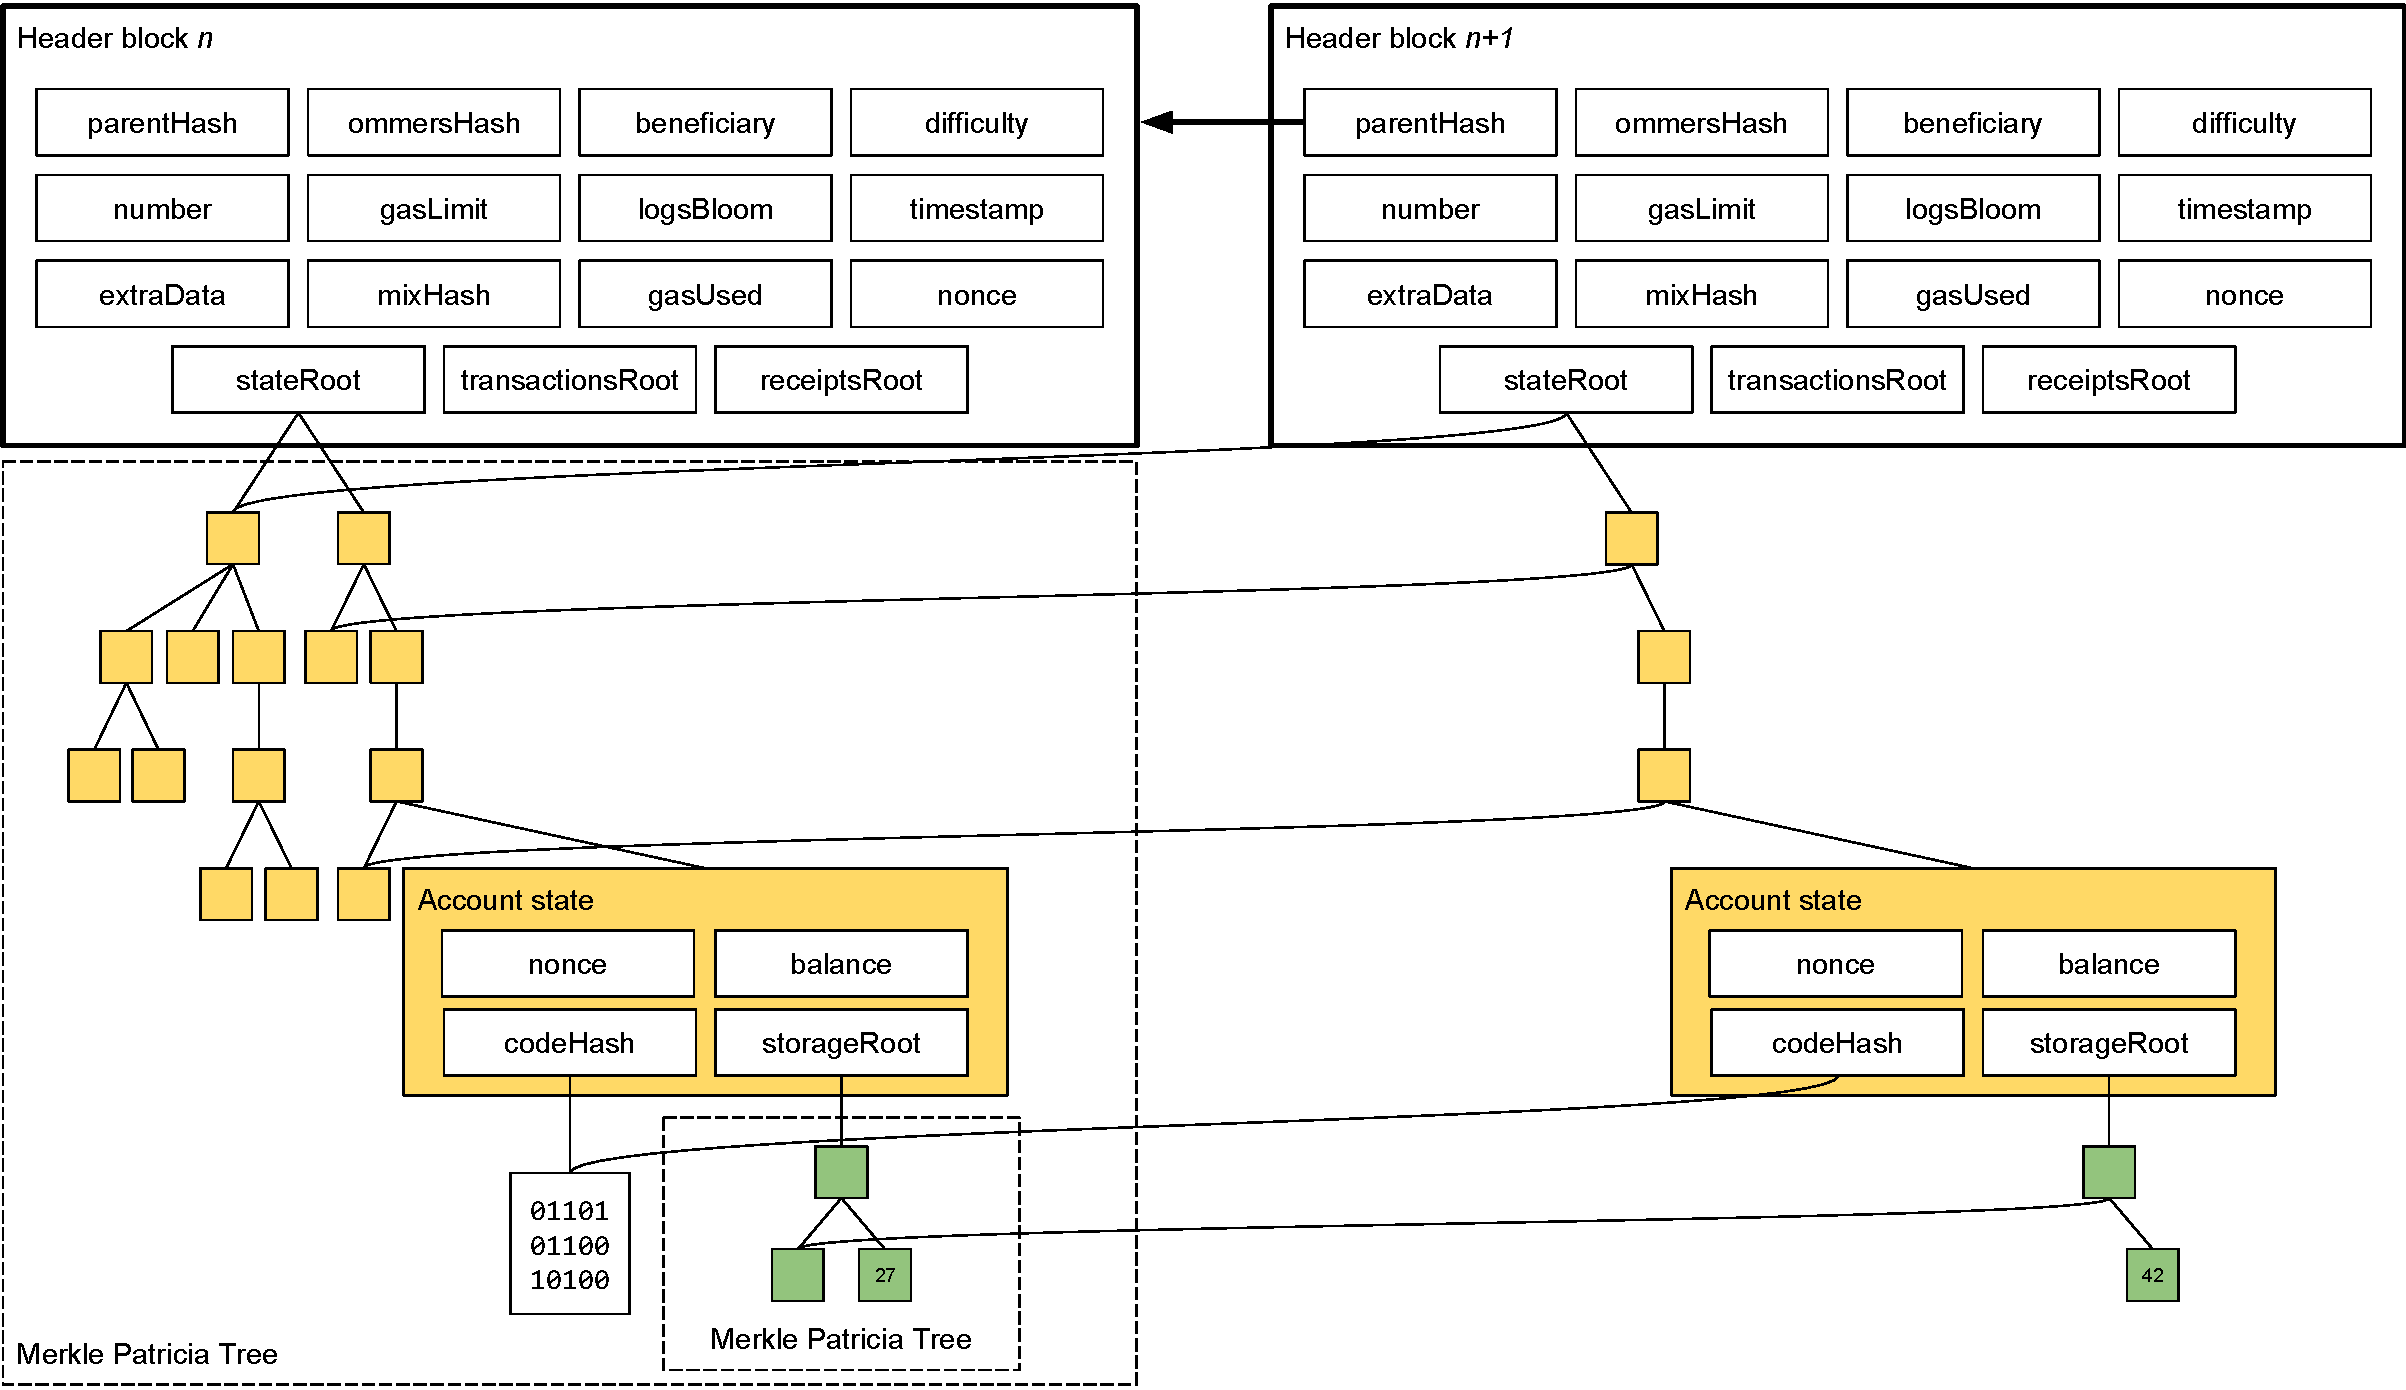
\includegraphics[width=\textwidth]{./res/img/world-state.pdf}
  \captionsource{Representation of the World State.}{Adapted from \url{https://ethereum.stackexchange.com/a/757}}
\label{fig:world-state}
\end{figure}

\autoref{fig:world-state} represents it. The block header contains 15 fields,
among which the \verb+stateRoot+, the \verb+transactionsRoot+ and the
\verb+receiptsRoot+. All these three fields are a hash of the root of a Merkle
Patricia tree data structure:

\begin{itemize}
  \item the \verb+stateRoot+ represents the state tree, after that all the
  transactions are executed and the finalisations are applied (for a complete
  specification of the fields, refer to \cite{wood2018ethereum}), storing the
  mapping between account state and account address
  \item the \verb+transactionsRoot+ represents the list of the transactions
  included in the block
  \item the \verb+receiptsRoot+ represents the receipts list of the transactions
  included in the block, which shows the \emph{effect} of each transaction. In
  \cite{merklingethereum}, the Ethereum's founder Vitalik Buterin writes that
  with the receipt information someone can answer queries like ``Tell me all
  instances of an event of type X (e.g. a crowdfunding contract reaching its
  goal) emitted by this address in the past 30 days''.
\end{itemize}

Some other block header fields are described in \autoref{sec:tests}. For a
complete fields list and description, we refer to the Ethereum protocol
specification~\cite{wood2018ethereum}.

\paragraph{Merkle Patricia tree}
A Merkle Patricia tree is a data structure which derives from a radix tree
reducing the space complexity \cite{patriciatree}. It has a single root, each
node is the hash of its children and the leaves are the actual data, that is,
for the case of the \verb+stateRoot+, the accounts states, which in turn include
the \verb+storageRoot+, a hash of another Merkle Patricia tree representing the
storage contents of the account state.

Since each node is the hash of its children, if any data in the tree changes,
recursively and correspondingly all the ancestors nodes have to change from the
changed node to the root node. This property allows to uniquely identify a tree
having just the root node. This is worth to notice because it allows the nodes
of the network to verify that big data structures (like the World State)
correspond to the one contained in the blocks' header by simply comparing a
$256$-bit long hash. Moreover, this feature can be exploited to create the light
nodes as described in~\autoref{sec:node-types}.


\subsubsection{Accounts}
\label{sec:accounts}

The accounts are also called the \emph{state objects} and are essential for the
user to interact with the Ethereum blockchain via transactions.

There are two types of accounts:

\begin{itemize}
  \item \textbf{Externally Owned Account} (EOA) (also referred to as simply
  \emph{account} or \emph{non-contract} account)
  \item \textbf{contract account} (also referred to as \emph{contract}), which
  has EVM Code associated with it and is controlled by its contract code.
\end{itemize}

An \emph{EOA} has no EVM Code associated with it and is controlled by a private
key. This type of account can send a message to another EOA, that is a value
transfer, or to a contract account in order to trigger the execution of code.
The state of an account is essentially its balance.

A \emph{contract account} has EVM Code associated with it and is controlled by
it. This type of account cannot send messages or transactions on its own, but
only as a response to a trigger. The state of a contract is its balance and its
contract storage. A contract code is executed by the EVM, can manipulate its own
persistent storage and can send internal transactions (i.e. message calls) to
other contracts.

Both the types of account have an associated \emph{nonce}. In the case of an
externally owned account this value corresponds to the number of transactions
sent by the account while in the case of a contract account it corresponds to
the number of contract creations performed by the account. Obviously, this value
is always positive and can only be increased.

When creating a transaction, the EOA should specify its nonce. This guarantees
that the order of transactions of a single account are processed in the order
specified by the sender. Without this expedient something unforeseen can happen,
for example, the balance of the account can get under a certain threshold and so
other transactions cannot be performed. Since contracts cannot perform
transactions but can still create other contracts once invoked, the nonce is
used to guarantee that each different created account have a different contract
address. Indeed, the contract address is obtained as function of the address of
the creator and its nonce~\cite{wood2018ethereum}.
